\chapter{The Inhabited Library}

\vspace{1em}
\hfill
\begin{minipage}[c]{0.55\textwidth}
\raggedleft
\small\itshape
The world is everything that is the case.\\[0.5em]
\upshape\footnotesize Ludwig Wittgenstein, \textit{Tractatus Logico-Philosophicus} (1921)
\end{minipage}%
\hspace{0.5em}
\begin{minipage}[c]{0.12\textwidth}
% \includegraphics[width=\textwidth]{figures/ch07_inhabited.png}
\end{minipage}
\vspace{1.5em}

\noindent Chapter 6 made the slip. The universal prior is now a measure on realities, not just on hypotheses. The Library contains every computable structure as a real thing.

What follows is the picture the slip gives you, an older question the picture sharpens, and the honest limits of any of it.

\section*{What both moves give}

With Moves I and II taken, the picture becomes:

The Library contains every computable reality. The universal prior $M$ is a measure on it. Your data restricts you to the subset of realities consistent with what you have observed. The measure on that subset describes which reality is yours, weighted by how plausible each candidate is.

You exist at many indices in the Library, in this picture. The pattern that constitutes your situation is instantiated wherever the structure of your situation occurs. Most of those instantiations are in universes with simple laws. A vanishingly small number are in universes whose laws are pathological. The universal prior tells you the proportions.

\begin{figure}[h]
\centering
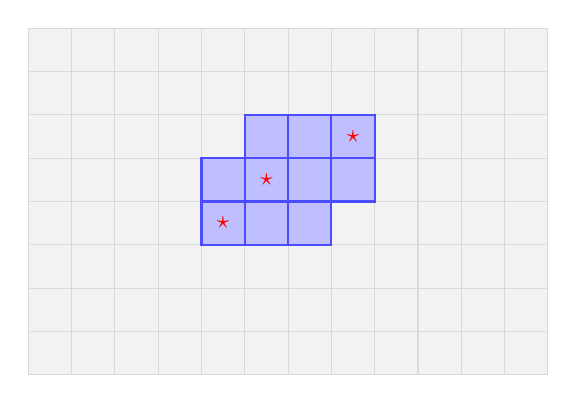
\begin{tikzpicture}[scale=0.55]
  % The Library: large grid of universes
  \foreach \x in {0,1,...,11} {
    \foreach \y in {0,1,...,7} {
      \draw[gray!30, fill=gray!10] (\x, \y) rectangle ({\x+1}, {\y+1});
    }
  }

  % Subset consistent with your data (blue cells)
  \foreach \x/\y in {4/3, 5/3, 6/3, 4/4, 5/4, 6/4, 7/4, 5/5, 6/5, 7/5} {
    \draw[thick, blue!70, fill=blue!25] (\x, \y) rectangle ({\x+1}, {\y+1});
  }

  % Mark "you" at several positions within subset
  \foreach \x/\y in {4/3, 5/4, 7/5} {
    \node[font=\small\bfseries, red] at ({\x+0.5}, {\y+0.5}) {$\star$};
  }
\end{tikzpicture}
\caption{What both moves give. Gray cells: the Library of all computable realities. Blue cells: the subset of realities consistent with your data. Red stars: indices at which the pattern that constitutes ``you'' is instantiated. The indexing question becomes measure-theoretic. The universal prior gives proportions, not a unique answer.}
\label{fig:multiplicity}
\end{figure}

The question \emph{where am I?} becomes measure-theoretic. It does not have a unique answer. It has a distribution.

\section*{An older question}

A reader who has followed this far may have an older question waiting. \emph{Why is there something rather than nothing?}

The question seems to assume that nothing is the simpler option. The chapter's tools do not directly settle this. Nothing, taken seriously, is the empty set: every possibility excluded. Like the universal set, it is informationally cheap. Both extremes have low description length. They are, in a sense, complements of the same kind of thing.

\begin{figure}[h]
\centering
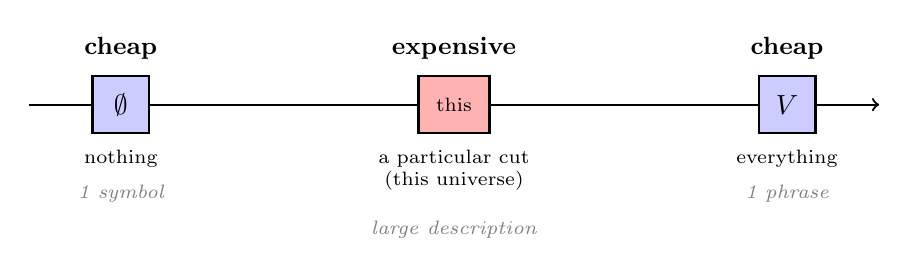
\begin{tikzpicture}[scale=0.9]
  % Horizontal axis line
  \draw[->, thick] (0, 0) -- (12, 0);

  % Position 1: ∅ (left end)
  \draw[thick, fill=blue!20] (0.9, -0.4) rectangle (1.7, 0.4);
  \node[font=\normalsize] at (1.3, 0) {$\emptyset$};
  \node[font=\scriptsize, anchor=north] at (1.3, -0.5) {nothing};
  \node[font=\scriptsize\itshape, gray, anchor=north] at (1.3, -1) {1 symbol};

  % Position 2: this universe (middle)
  \draw[thick, fill=red!30] (5.5, -0.4) rectangle (6.5, 0.4);
  \node[font=\scriptsize, align=center] at (6, 0) {this};
  \node[font=\scriptsize, anchor=north, text width=3.5cm, align=center] at (6, -0.5) {a particular cut (this universe)};
  \node[font=\scriptsize\itshape, gray, anchor=north] at (6, -1.5) {large description};

  % Position 3: V (right end)
  \draw[thick, fill=blue!20] (10.3, -0.4) rectangle (11.1, 0.4);
  \node[font=\normalsize] at (10.7, 0) {$V$};
  \node[font=\scriptsize, anchor=north] at (10.7, -0.5) {everything};
  \node[font=\scriptsize\itshape, gray, anchor=north] at (10.7, -1) {1 phrase};

  % Top labels
  \node[font=\small\bfseries] at (1.3, 0.8) {cheap};
  \node[font=\small\bfseries] at (6, 0.8) {expensive};
  \node[font=\small\bfseries] at (10.7, 0.8) {cheap};
\end{tikzpicture}
\caption{The endpoints and the cut. The empty set and the universal set are both informationally cheap, describable in a phrase. A specific intermediate cut (such as ``this particular universe'') requires substantial information. The cost lives in the cut, not in the totality. Nothing and everything are, by this measure, on equal footing.}
\label{fig:endpoint-spectrum}
\end{figure}

So the cut principle does not, by itself, favor either nothing or something. Both are cheap.

What does favor something: we observe it.

You are reading these words. Something exists. This is not a metaphysical assumption; it is the data. Any theory of reality that predicts no existence at all is immediately falsified by the existence of the observer. The nothing-hypothesis is excluded by induction on the only sample available, which is the entirety of what anyone has ever observed.

The induction operates one level above the within-universe inductions of earlier chapters. We are not asking which universe is ours within the Library. We are asking which kind of generator generates realities at all. The nothing-generator generates none. We are in a reality. The nothing-generator is empirically excluded.

There is also a coherence question. Is \emph{nothing} a position one could coherently hold?

To say nothing exists is to say no possibilities are realized. The claim presupposes a domain of possibilities from which the realized ones are absent. But if nothing exists, no domain exists either. There are no possibilities to be absent. The very concept of an excluded possibility seems to require a background of possibilities to exclude from.

The concept of nothing may quietly require the concept of something to mean anything at all. It may not pick out a coherent position so much as the limit of a concept that breaks down before reaching it.

The book does not resolve this. The note is here because it is honest. The cut principle does not by itself rule out nothing on simplicity grounds; observation does. And on close inspection, nothing may not be a coherent option at all.

\section*{What if you refuse}

The book takes both moves. The reader does not have to.

Refuse Move I, and the universal prior remains the right epistemic prior. Cox's theorem, Kraft's inequality, Solomonoff's dominance theorem all still apply. The mathematics of optimal learning is unchanged. What you cannot say is that the prior tells you anything about reality. It tells you about belief.

Refuse Move II, and Move I survives. The universe is computable; there is one of it; the universal prior is the right prior over the one. Multiplicity does not enter.

Many of the implications in Part II of this book survive in either of these reduced positions. The dissolution of the unitary self temporally (the way \textit{Worldlines} treated it) does not require Move II. The discipline of attention, the practice of care, the response to indifference: all of these survive without the multiverse picture.

The questions that specifically require multiplicity (quantum immortality, the dissolution of the self \emph{across} branches, the Boltzmann brain problem) require Move II or some other route to a multiverse.

The book labels which conclusions follow from which moves. The cascade can always be unwound. A claim that requires Move II is marked as such. A claim that requires only Move I is marked as such. A claim that follows from bedrock alone is unmarked, because it is settled. The reader can trace any conclusion back to the move it depends on and refuse the move if the conclusion is unwelcome.

This is the structure of honesty the book commits to.

\section*{Where this leaves you}

The slip has been made and its picture has been drawn. The Library has been read ontologically. Multiplicity, in this picture, is a structural fact rather than a thought experiment.

The next chapter takes a second route to the same place. Quantum mechanics, on its cleanest interpretation, also produces a multiverse, by a path that does not invoke CUH. Two independent moves arriving at the same picture is convergent evidence that the picture is not arbitrary.

Two routes to the same Library.
